
\section{Algorithme} \label{title-lbm_algo}
Pour simuler le comportement de fluides, \acs{LBM} découpe l'espace physique à modéliser en un domaine discret composé de populations, organisées en une grille, et discrétise le temps en générations. 

Une population représente une portion de l'espace physique. Une simulation consiste en l'application de deux étapes de calculs, effectuées de façon identique sur chaque population du domaine, pour calculer les populations de la génération suivante où le processus pourra être répété. Le résultat de la génération $t$ ne dépend par conséquent que de l'état du domaine à la génération $t-1$.  Il s'agit, à l'instar du bien connu jeu de la vie de \textsc{J.~Conway}, d'un automate cellulaire.


Une population, illustrée par la figure \ref{fig:population_d2q9}, est composée de 9 directions (nord, sud, est ...), auxquelles sont attribuées une valeur qui représente la densité de probabilité qu'a la vélocité du fluide d'aller dans une direction donnée et un ordre arbitraire, à travers une numérotation (pour simplifier les formules).

\begin{figure}[h]
	\centering
	\subfigure[Directions]{%
		\centering
		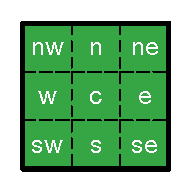
\includegraphics[scale=1]{images/population.pdf}
	}
	\subfigure[Numérotation]{%
		\centering
		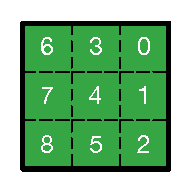
\includegraphics[scale=1]{images/population_numerotation.pdf}
	}
	\caption{Population D2Q9}
	\label{fig:population_d2q9}
\end{figure}
Les populations du domaine sont notées $f^{in}(x,t) = \{f^{in}_0(x,t), f^{in}_1(x,t), \dots f^{in}_8(x,t)\}$, avec $x$ la position dans la grille.

La première étape de simulation d'une génération, dite de \textit{collision}, introduit les vecteurs de vélocité $v$,  tel que les voisins de $f^{in}(x, t)$ sont trouvés par $f^{in}(x+v_i,t)$: 
\begin{multicols}{3}
\begin{itemize}
\item[] $v_0 = [1,1]$
\item[] $v_1 = [1,0]$
\item[] $v_2 = [1,-1]$
\item[] $v_3 = [0,1]$
\item[] $v_4 = [0,0]$
\item[] $v_5 = [0,-1]$
\item[] $v_6 = [-1,1]$
\item[] $v_7 = [-1,0]$
\item[] $v_8 = [-1,-1]$
\end{itemize}
\end{multicols}

On commence par calculer les variables \textit{macroscopiques} de la population, soit sa densité $\rho$ et ses vélocités $u$:\\[-2\baselineskip]
\begin{multicols}{2}
\begin{equation}
\rho(x, t) = \sum_{i=0}^{8} f^{in}_i(x,t)
\end{equation}
\begin{equation}
u = \frac{1}{\rho(x,t)}\sum_{i=0}^{8} v_i \cdot f^{in}_i(x,t)
\end{equation}
\end{multicols}~\\[-0.5\baselineskip]
\noindent puis on calcule les directions $i$ de la population $f^{out}$ qui résultent de la collision:
\begin{equation}
f^{out}_i = f^{in}_i - \omega \cdot \big(f^{in}_i - E(i, \rho, u) \big)
\end{equation}

\noindent avec $E$ la fonction d'\textit{equilibrium}:
\begin{equation}
E(i, \rho, u) = \rho\cdot t_i \bigg(  1 + \frac{v_i \cdot u}{c^2_s} + \frac{1}{2~c^4_s} (v_i \cdot u)^2 - \frac{1}{2~c^2_s} |u|^2 \bigg)
\end{equation}\\[-\baselineskip]

\noindent avec $c_s$ la vitesse du son, $\omega$ le paramètre de relaxation, et les constantes $t_i$, qui compense les longueurs inégales des différentes vélocités, avec $t_i = \nicefrac{1}{9}$ pour les directions orthogonales, $t_i =\nicefrac{1}{36}$ pour les diagonales et $t_i=\nicefrac{4}{9}$ pour la centrale, soit:

\begin{equation}
t = \{\nicefrac{1}{36} , \nicefrac{1}{9}, \nicefrac{1}{36}, \nicefrac{1}{9}, \nicefrac{4}{9}, \nicefrac{1}{9}, \nicefrac{1}{36}, \nicefrac{1}{9}, \nicefrac{1}{36}\}
\end{equation}\\[-\baselineskip]

La seconde étape, illustrée par la figure \ref{fig:population_streaming}, propage les densités des populations $f^{out}$ calculées dans cette génération $t$ dans les nouvelles populations de la suivante $t+\delta t$, où $\delta t$ correspond au pas de temps utilisé.

\begin{equation}
f^{in}_i(x,t) = f^{out}_i(x-v_i\delta t, t - \delta t)
\end{equation}\\[-\baselineskip]

On observe dans ce processus qu'il est hautement parallélisable. Chaque population est calculée indépendamment des autres, jusqu'à la propagation qui n'implique que les voisins directs de la cellule. C'est ce potentiel qu'exploitent les implémentations parallèles, pour accélérer leur simulation.

\begin{figure}[H]
	\centering
	\subfigure[Génération $t$]{%
		\centering
		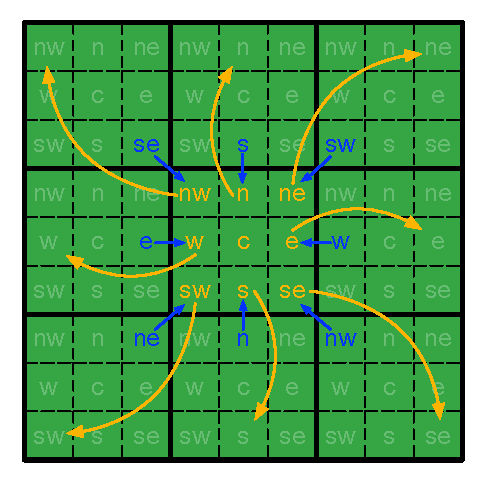
\includegraphics[scale=0.8995]{images/pre-streaming.pdf}
	}
	\subfigure[Génération $t+\delta t$]{%
		\centering
		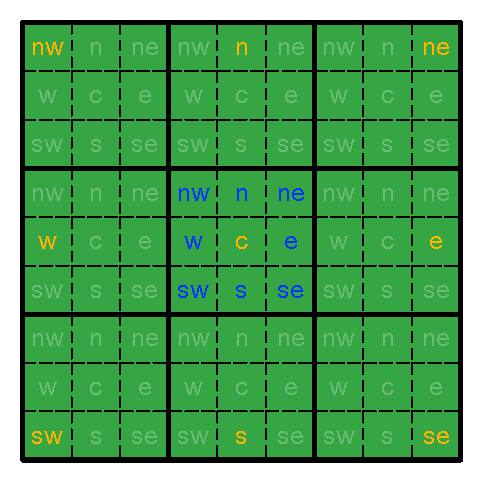
\includegraphics[scale=0.8995]{images/post-streaming.pdf}
	}
	\caption{Propagation pour la population $f^{in}(x,t)$ au centre ($x=[1,1]$) }
	\label{fig:population_streaming}
\end{figure}

\section{Notation DnQm}
L'algorithme présenté dans la section \ref{title-lbm_algo} est axé sur un domaine en 2 dimensions, et avec des populations à 9 directions. On note cette configuration D2Q9, avec D2 pour le nombre de dimensions et Q9 le nombre de directions. 

En effet, l'algorithme est également applicable pour 3 dimensions, avec les configurations D3Q15, D3Q19 et D3Q27.

\section{Unité de mesure de performance LUPS}

La simulation de fluide avec \acs{LBM} est un processus gourmand en mémoire et en temps de calcul. Un pan important de la recherche concernant \acs{LBM} vise à trouver des techniques pour améliorer les performances de son implémentation.

Les \acl{LUPS} (populations calculées par seconde) ou \XLUPS{} sont communément utilisés comme unité de mesure des performances.